\documentclass[]{article}
\usepackage{graphicx}
\usepackage{hyperref}
\usepackage{amsmath}
\usepackage{caption}
\usepackage{subcaption}

%opening
\title{Dynamic Light Scattering}
\author{Gunther T\"urk, Jonas Lehnen}

\begin{document}

\maketitle
\tableofcontents
\begin{abstract}
In this experiment we want to get informations about the properties of our samples by scattering light on them. Just like in nuclear physics we are able to conclude how a particle looks like by measuring the lights intensity depending on the scattering angle. Furthermore, we are interested in how long an particles movement is coherent to itself. With this information we are able to determine the Stokes radius and compare it with the radius resulting from the form factor.


Write here, what we did and learned.
\end{abstract}


\section{Theorie}
\subsection{Colloids}
Colloids are small particles, but still $10^3$ to $10^4$ times larger than an atom, which are dissolved in a dispersion medium. Depending on the aggregation of state the colloidal systems are named differently. Liquid in a gaseous medium is called liquid aerosol while 2 liquids combined are called emulsion. Examples are mist and steam as well milk and salad dressing.

%Ist der part drunter so richtig?
Colloids are often spherical shaped and tend to aggregate with each other. This is preventable by stabilisation techniques. The electrostatic stabilization is creatable when a colloid with groups like $~OH$ or $~SO_3H$ are dissolved in a liquid. These groups  can then dissociate as ions and the colloid becomes negatively charged with a cloud of positive ions around it. Now the colloids are repulsing each other due to their equally charged clouds. For high salt concentrations e.g. $NaCl$ this effect is reduced. The increased amount of ions caused by the dissolved salt prevents the colloids separation of charge and with this the repulsion between colloids is reduced. 
The steric stabilisation creates this repulsive force via polymers on the colloids surface. These are preventing the aggregation by keeping them apart.

Depending on particle density $n_p$ in a constant volume $V$ one can define the volume fraction $\Phi = n_p \cdot V$. This corresponds to the change of phase in a colloidal system. For a system with hard spheres the crystallization form liquid starts at $\Phi=0.494$ if the increase happens in equilibrium. For a more rapid process without equilibrium the glass phase is reachable. This happens if your system freezes nearly instantaneously.  

\subsection{Light Scattering}
Considering quasi-elastic light scattering, a photon gets absorbed by a scattering center, induces a dipole moment and gets re-emitted in a different angle. The length of the wave vector $ |\vec{k}| = \frac{2\pi n}{\lambda}$ and therefore the energy do not change in this assumption. So the momentum change for a single photon is given by:
\begin{equation}\label{eq:momentum}
q= |\vec{k_{in}} - \vec{k_{out}}| = \frac{4\pi n}{\lambda} \cdot \sin \left( \dfrac{\Theta}{2} \right)  
\end{equation}

\paragraph{Born approximation}\mbox{}\\
In the Bron approximation we basically assume that every particle scattering light emits a spherical wave which is not scattered further. This assumption is fine for highly dilute samples.
Using the Born approximation, we neglect every induced fields from the dipole oscillation which would again induce others molecules to oscillate. These oscillations would change our scattered light.% Born approximation erklären
%Hab ich glaub ich gemacht

The lasers wavelength is nearly as large as our colloids. Therefore we're not allowed to use the approximation of Rayleigh scattering. By considering every colloid as its own scattering centre we now can conclude how the particles are distributed in the system.

In the experiment intensity is measured. From the conclusion above we can derive a formula, just depending on the form factor $P(q)$ given by the size of the individual colloids and how they are arranged in the medium:
\begin{equation} \label{eq:intensity}
I(q) = I_0(q)b(\vec{q}=0)^2 \cdot P(q) \cdot NS(q)
\end{equation}
Where N is the number of colloids in the system and b(q) 
% was genau stellt b dar, außer komisches Ergebnis aus der Integration
%Fouriertransformierte der größe des teilchens?
\\

\begin{equation}\label{eq:form}
P(q)= \frac{9}{(qa)^6} \cdot (sin(qa) - qa \cdot cos(qa))
\end{equation}


For moving particles their dynamics are getting important. Due to Brownian motion, see \ref{hyd}, the correlation of the electric field to itself at a later time is affected. One defines the autocorrelation function 
\begin{equation}\label{eq:g1}
G_1(\vec{q}) = \langle \: \vec{E}(\vec{q},t),\vec{E}(\vec{q},t+\tau) \: \rangle
\end{equation} 
Because we are only able to measure the intensity of light we need a connection to the autocorrelation of the electric field. It can be derived by simple calculation and is called the Siegert relation:
\begin{equation}\label{eq:siegert}
g_2(\vec{q},t) = g_1(\vec{q},t )^2 +1
\end{equation}
where $g_2$ is the normalized autocorrelation of the intensity. For highly dilute samples we can further calculate $g_1$ with Fick's second law
\begin{equation}\label{eq:g1solved}
g_1(\vec{q},t )=e^{-\vec{q}^{2}D_0*\tau}
\end{equation}
where $D_0$ is the Diffusion coefficient defined as 
\begin{equation}\label{eq:StokesEinstein}
D_0=\frac{k_BT}{6\pi \eta a}
\end{equation}
This finally gives us 
\begin{equation}\label{eq:g2}
\boxed{g_2(\vec{q},t) =e^{- \vec{q}^{2}}D_0*\tau+1}
\end{equation}
for our measured autocorrelation. We are therefore able to measure the hydrodynamic radius "a" of the colloids in our samples.


\subsection{Hydrodynamics}
\label{hyd}
First of all we introduce the material constant viscosity. It describes how strong the friction is for moving something through a medium. Usually it's defined as: 
\begin{equation}
\vec{F}=\eta A \frac{\partial \vec{v}}{\partial x} , \quad \eta(T)= \eta_0 e^{\frac{E_A}{RT}}
\end{equation}
\subsubsection{Brownian motion}
Brownian motion describes the random movement of microscopic particles in liquids and gases. According to kinetic gas theory molecules in a gas or a liquid are in constant isotrop motion, that we can measure as temperature. These particles randomly hit the much larger colloids or other microscopic particles, causing a change in momentum. This change in momentum causes a what looks like a wiggling motion of the microscopic particles. The Brownian motion therefore increases with temperature cause the average momentum of the molecules is hitting the microscopic particles is larger.
%thermische bewegung der moleküle wegen T fehlt noch

\subsubsection{Stokes law and hydrodynamic radius}
%Erklären was hydrodynamic radius ist fehlt noch und vgl. mit el.dyn radius
Stokes law gives a simple relation to determine the viscosity of a liquid. It gives us the force needed to move a spherical object with the hydrodynamic radius a through a liquid with the velocity $\vec{v}$. The proportionality between these is the viscosity.
\begin{equation}\label{eq:Stokes}
	\vec{F}_s=6 \pi \eta a \vec{v_s}
\end{equation}
To experimentally determine the viscosity of a liquid you drop a sphere with a known mass in the liquid and measure the terminal velocity. There $\vec{F_s}+\vec{F_{lift}}=\vec{F{gravitaion}}$ so we can determine the viscosity to be
\begin{equation}
	\eta=\frac{2(\rho_{sphere}-\rho_{liquid})g  a^2}{9v_s}
\end{equation} 


\subsubsection{Diffusion}
Thermodynamics tells us that a system of particles always goes to the state with the highest entropy. For a system consisting of two different particles this is accomplished by an equal distribution of the two particles over the entire system. The process which causes this equilibrium is called diffusion. It is described by Fick's laws, where J is the flow of particles, $\frac{dc}{dx} $ is the concentration gradient and D is the diffusion coefficient. 
\[ J=-D\frac{dc}{dx}\]
We can see that the particles flow towards the point with the lowest concentration and that the speed of diffusion depends on the diffusion coefficient.

\subsection{Laser and Photomultiplier}
In the experiment we are using a green $532nm$. The main principles for a laser are the inversion and the stimulated emission. Considering a 3 state energy system. Inversion is created by pumping nearly every electron from the ground state into the most excited state, this means sending in photons with the transition frequency as energy. This frequency is only for the pumping and usually higher than the lasers one. The most excited state should decay fast to the middle state that should have a long lifetime. There the electrons will wait for a photon in laser frequency to stimulate the emission of an exact identically photon. This means we end up with a electron in the ground state and two photons instead of one. Due to their same properties, i.e. same frequency and phase relation to each other, a laser creates coherent light.

The function of a photomultiplier relies on the photoelectric effect. Hereby a photon collides with a cathode and triggers an electron to leave the material.
Due to a increasing potential between the cathode and the following dynodes the electron will always hit the next potentially higher dynode. Thereby it gains more speed and is able to knock more electrons out of the dynode. Due to their shape the electrons won't skip any dynode and the amount of electrons travelling increases exponentially this the amount of dynodes. At the end they'll get absorbed from the anode to measure the current and thereby getting a signal that the cathode was hit by a photon.

\newpage
\section{Experiment}
\subsection{Setup}
The following figure shows how the basic arrangement of hardware was. Everything was controllable by the given software. Except the sample change had to be done manually. The positioning of the sample was a little bit difficult. The holder was only a small hole in a cap for the isopropyl alcohol container and the sample was placed by the friction with this hole. We tried to align it straight downwards, but it could have been tilted. The refractive index of isopropyl alcohol is $n=1.37927$ for $T=293K$. The measured temperature for the sample was $19.6 ^\circ C$ with an digital infra-red thermometer. Therefore we are using the literature value as given above.

\begin{figure}[!htbp]
\centering
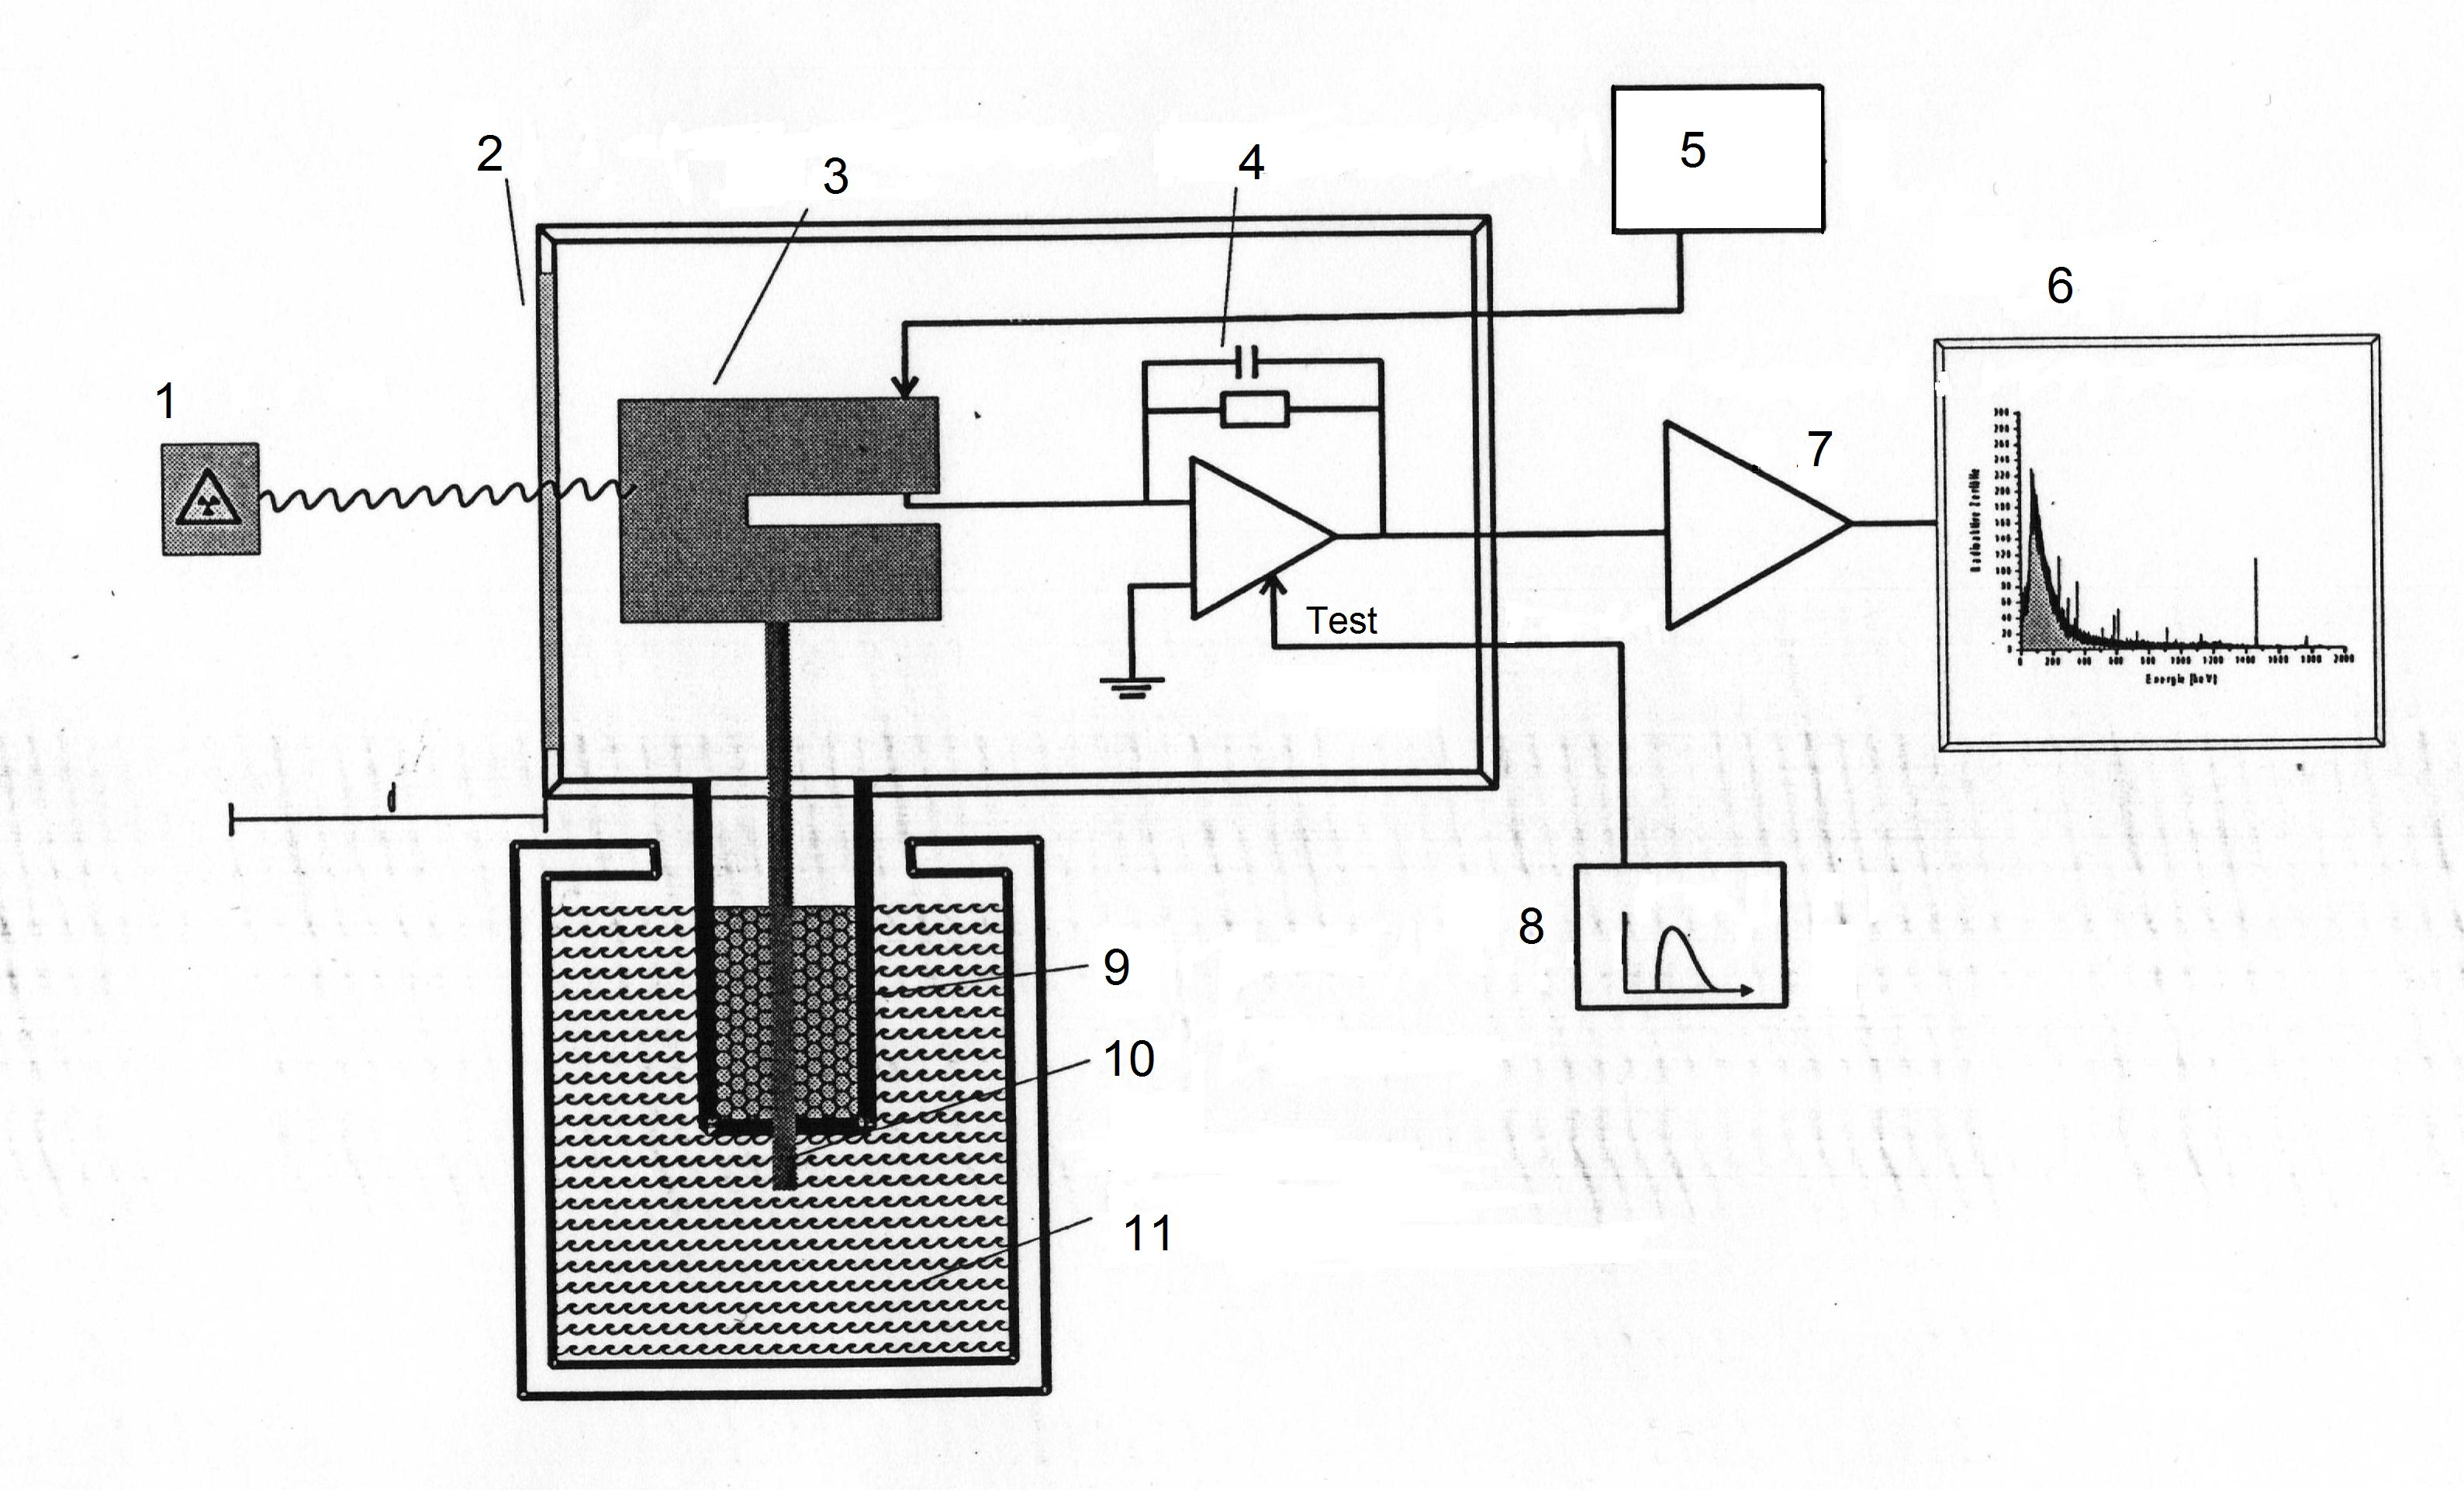
\includegraphics[width=0.8\linewidth]{Plots/Setup.png}
\caption{The experimental Set-up for our the Dynamic Light Scattering experiment. Figure taken from the given script.}
\end{figure}

We used green $532nm$ laser light for the scattering at the samples. To avoid static installations and prevent displacements in the lights path, optical fibres were used. The goniometer itself was purely adjustable by electronics to get an exact angle measurement.


\subsection{A: Small particles in fluid phase}
\subsubsection{Form factor}

For fitting the form factor of the colloids we'll use equation (\ref{eq:intensity}). Thereby we introduce another constant value A in (\ref{eq:form}) which absorbs everything factor independent of q this means except of $P(q)$ and $S(q)$. The structure function is nearly 1 for very dilute samples. The assumption that there are very few colloids in the medium is justified because we couldn't see any real particles with the naked eye. 

\begin{figure}[!htbp]
\centering
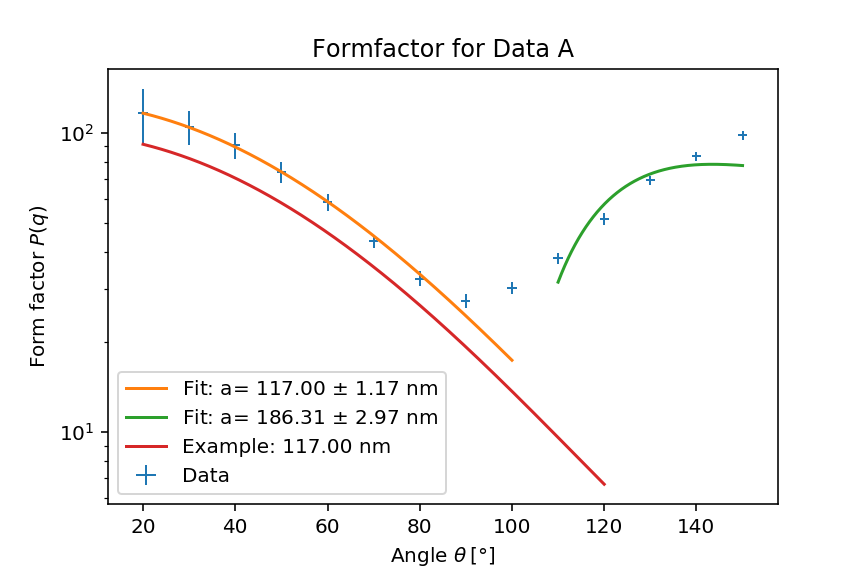
\includegraphics[width=0.8\linewidth]{Plots/FormA.png}
\caption{Intensity fitted for the form factor.}
\label{FormA}
\end{figure}

Before fitting the intensity has to be corrected. Due to the change in momentum related to the scattering angle. To get the angle independent intensity our measured mean intensities has to be multiplied by $sin(\frac{\theta}{2} )$.
Fitting only fractions of the measured values results as pictured in better fitting curves. They're always displayed for the used values. Their radii are now much larger than expected. But as pictured in "Example" the curves don't continue with fitting nearly perfectly. This curve is just for comparison reasons and is shown with a small offset so it does not disturb the other graphs.

Now looking at Figure \ref{FormA}. The first fit includes every point and does not look like the function describing our data. Although its result is only off by a factor of 2 compared to the given particle radius of $35nm$. 

We also tried to fit for a form function for a polydisperse distributed in a Gaussian with $\mu$ as the given particle radii. 
\[ \overline{P(q)} = \int_0^\infty da\: f(a)\cdot P(q,a) , \quad f(a)= \frac{1}{\sqrt{2 \pi \sigma^2}} e^{-\frac{(a-\mu)^2}{2 \sigma^2}} \]
But the integration already failed for a test value. For expected radii between $35$ and $180nm$ and values of momentum transfer with the lasers wavelength, the returned values didn't change from zero. 

\subsubsection{Hydrodynamic radius and diffusion coefficient}
We measured the autocorrelation for every sample and in case of sample A and B for angles between 20$^\circ$ and $150^\circ$ in steps of 10$^\circ$ and fitted the parameter $D_0$ of $g_2$ (\ref{eq:g2}) to our data (e.g. fig.  \ref{fig:Sample A 60}). This way we were able to calculate the hydrodynamic radius of the colloids in our sample with the Stokes-Einstein-relation (\ref{eq:StokesEinstein}) This gave us an average radius of $62.49 nm$. This fits quite well the actual radius of the colloids of $35nm$. As expected the  hydrodynamic radius is slightly larger than the actual radius. 

%Hier muss noch der vgl der daten des hydrodyn radius und dem formfaktor hin... passt nicht mit unseren daten aber mit 35nm die er uns gegeben hat


\begin{figure}
	\centering
	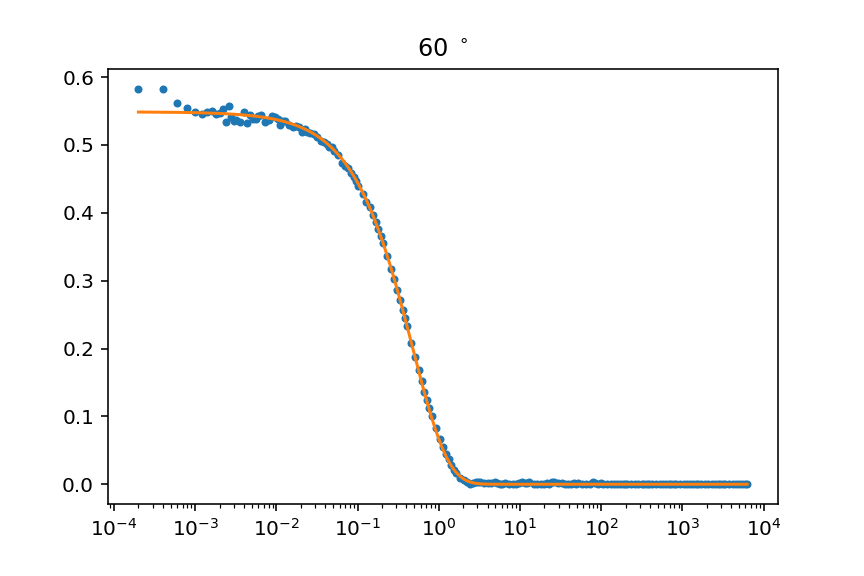
\includegraphics[width=0.7\linewidth]{Plots/A/60}
	\caption[Autocorrelation with fit of $g_2$]{}
	\caption{Example of the autocorrelation with fit. For more see Appendix.}
	\label{fig:Sample A 60}
\end{figure}

%Tabelle einfügen
\begin{table}[h]
	\centering
	\begin{tabular}{|c|c|c|c|c|c|}
		\hline
		D & dD & a & da & q & angle \\ \hline\hline
		3.99e-15 & 2.55e-17 & 6.16e-08 & 3.95e-10 & 5.66e+06 & 20 \\ \hline
		4.03e-15 & 1.24e-17 & 6.10e-08 & 1.88e-10 & 8.43e+06 & 30 \\ \hline
		3.89e-15 & 1.49e-17 & 6.32e-08 & 2.42e-10 & 1.11e+07 & 40 \\ \hline
		4.04e-15 & 1.45e-17 & 6.08e-08 & 2.18e-10 & 1.38e+07 & 50 \\ \hline
		3.97e-15 & 2.22e-17 & 6.19e-08 & 3.46e-10 & 1.63e+07 & 60 \\ \hline
		3.94e-15 & 2.14e-17 & 6.24e-08 & 3.39e-10 & 1.87e+07 & 70 \\ \hline
		3.84e-15 & 2.73e-17 & 6.40e-08 & 4.55e-10 & 2.09e+07 & 80 \\ \hline
		4.05e-15 & 5.72e-17 & 6.06e-08 & 8.57e-10 & 2.30e+07 & 90 \\ \hline
		3.96e-15 & 4.05e-17 & 6.21e-08 & 6.36e-10 & 2.50e+07 & 100 \\ \hline
		3.92e-15 & 2.90e-17 & 6.27e-08 & 4.65e-10 & 2.67e+07 & 110 \\ \hline
		3.89e-15 & 1.83e-17 & 6.32e-08 & 2.98e-10 & 2.82e+07 & 120 \\ \hline
		3.84e-15 & 1.50e-17 & 6.40e-08 & 2.50e-10 & 2.95e+07 & 130 \\ \hline
		3.86e-15 & 1.05e-17 & 6.36e-08 & 1.73e-10 & 3.06e+07 & 140 \\ \hline
		3.84e-15 & 6.78e-18 & 6.39e-08 & 1.13e-10 & 3.15e+07 & 150 \\ \hline
		\hline
	\end{tabular}
	\caption{A data}
	\label{tab:adata}
\end{table}



\subsection{B: Large particles in fluid phase}
\subsubsection{Form factor}
Again we tried to to fit for P(q). With the same procedure figure \ref{FormB} is created. Again the partial fits are good looking for their individual space but the whole fit is completely off.

Sample B was supposed to have a five times larger colloid radius than A. We performed the same measurements and expected getting different values for the scattering radius as well as the hydrodynamic radius. 
We calculated an average hydrodynamic radius of $51 nm$. 



%Bdata
\begin{table}[h]
	\centering
	\begin{tabular}{|c|c|c|c|c|c|}
		\hline
		D & dD & a & da & q & angle \\ \hline\hline
		4.80e-15 & 5.78e-17 & 5.11e-08 & 6.16e-10 & 5.66e+06 & 20 \\ \hline
		4.73e-15 & 2.59e-17 & 5.19e-08 & 2.84e-10 & 8.43e+06 & 30 \\ \hline
		4.54e-15 & 3.09e-17 & 5.41e-08 & 3.68e-10 & 1.11e+07 & 40 \\ \hline
		4.82e-15 & 2.69e-17 & 5.10e-08 & 2.85e-10 & 1.38e+07 & 50 \\ \hline
		4.75e-15 & 3.70e-17 & 5.17e-08 & 4.03e-10 & 1.63e+07 & 60 \\ \hline
		4.86e-15 & 5.72e-17 & 5.05e-08 & 5.94e-10 & 1.87e+07 & 70 \\ \hline
		4.97e-15 & 8.02e-17 & 4.94e-08 & 7.98e-10 & 2.09e+07 & 80 \\ \hline
		4.95e-15 & 8.58e-17 & 4.96e-08 & 8.61e-10 & 2.30e+07 & 90 \\ \hline
		4.93e-15 & 4.94e-17 & 4.98e-08 & 5.00e-10 & 2.50e+07 & 100 \\ \hline
		4.97e-15 & 7.14e-17 & 4.95e-08 & 7.11e-10 & 2.67e+07 & 110 \\ \hline
		4.75e-15 & 4.17e-17 & 5.17e-08 & 4.54e-10 & 2.82e+07 & 120 \\ \hline
		4.81e-15 & 2.58e-17 & 5.11e-08 & 2.74e-10 & 2.95e+07 & 130 \\ \hline
		4.74e-15 & 2.17e-17 & 5.18e-08 & 2.37e-10 & 3.06e+07 & 140 \\ \hline
		4.78e-15 & 1.35e-17 & 5.14e-08 & 1.45e-10 & 3.15e+07 & 150 \\ \hline
		\hline
	\end{tabular}
	\caption{B data}
	\label{tab:bdata}
\end{table}



\subsection{Comparison of samples A and B}
Contrary to our expectoration we measured a slightly smaller hydrodynamic radius for sample B. The most likely explanation for this is that the samples were not the ones described in the script. While we are sure to have changed the samples after the first measurement it is likely that sample B was just another tube with the sample A, because no sample was labelled and they looked very similar.

\begin{figure}[!htbp]
\centering
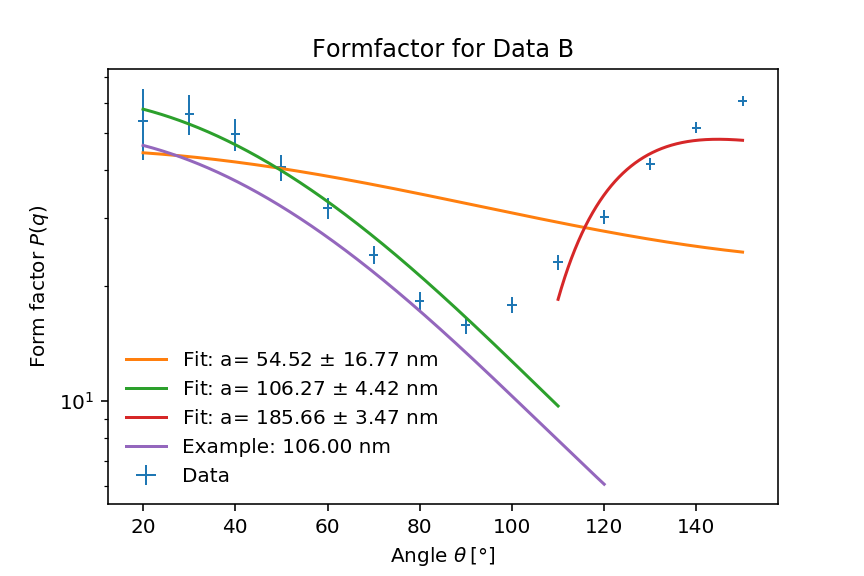
\includegraphics[width=0.8\linewidth]{Plots/FormB.png}
\caption{Intensity fitted for the form factor.}
\label{FormB}
\end{figure}

\subsection{C: Small particles in fluid phase, high concentration}

\begin{figure}[!htbp]
\centering
\includegraphics[width=0.8\linewidth]{Plots/"C bei 40".png}
\caption{Autocorrelation for the Sample C at 40 degrees.}
\label{C}
\end{figure}


\newpage
\subsection{D: Small particles in crystalline phase}
The last sample was clearly different from the other. One already could see a light white coloured gleam due to the high concentration which causes the crystalline phase. 

\begin{figure}[!htbp]
\centering
\includegraphics[width=0.8\linewidth]{Plots/"D bei 40".png}
\caption{Autocorrelation for the Sample D at 40 degrees. It shows a second slope which is caused by the newly formed crystalline structure in the medium.}
\label{D}
\end{figure}

As pictured in Figure \ref{D} a second slope appears for the crystalline phase. The high concentration forces the particles to come together and thereby form new structures which also causes the white gleam. These new structures are now larger than the usual particles moving in the medium. Thereby they will show a different decay time for the correlation of their momentum.


\newpage
\section{Appendix}

\subsection{Autocorrelation A}
\label{autocorr A}
\begin{figure}[!h]
\centering

\begin{subfigure}{0.48\textwidth}
\includegraphics[width=\linewidth]{Plots/A/20.png}
\end{subfigure}
\begin{subfigure}[c]{0.48\linewidth}
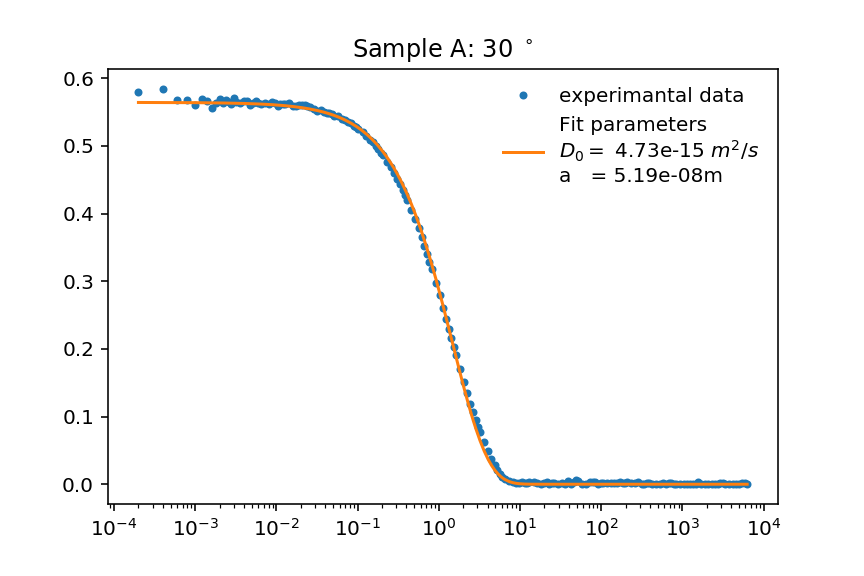
\includegraphics[width=\linewidth]{Plots/A/30.png}
\end{subfigure}

\medskip
\begin{subfigure}{0.48\textwidth}
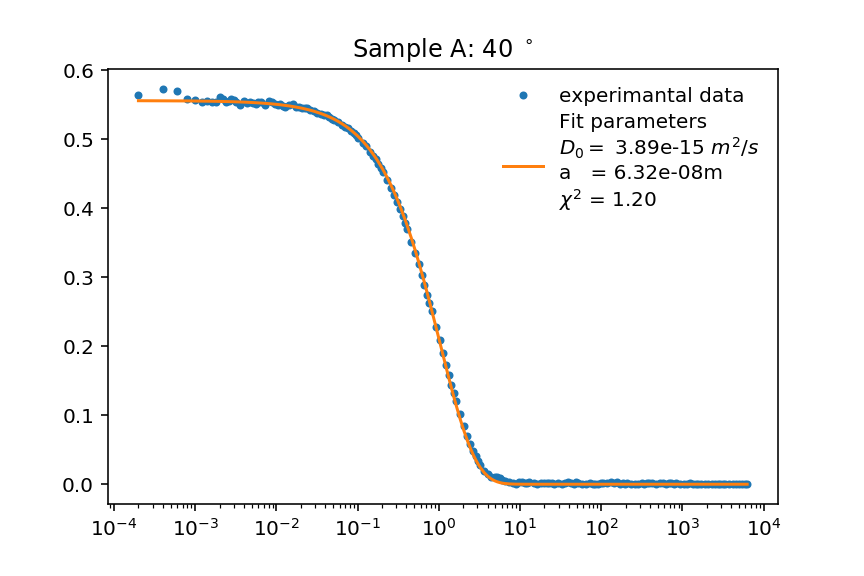
\includegraphics[width=\linewidth]{Plots/A/40.png}
\end{subfigure}
\begin{subfigure}[c]{0.48\linewidth}
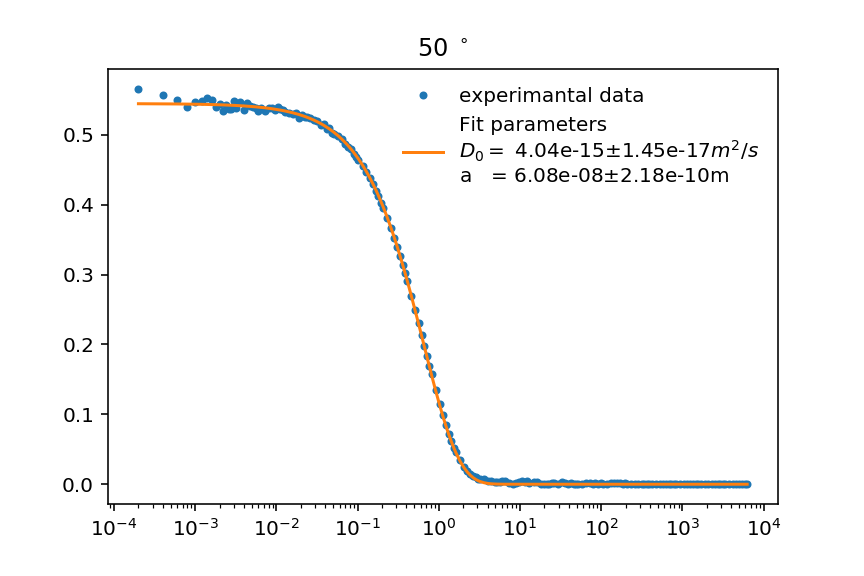
\includegraphics[width=\linewidth]{Plots/A/50.png}
\end{subfigure}

\medskip
\begin{subfigure}{0.48\textwidth}
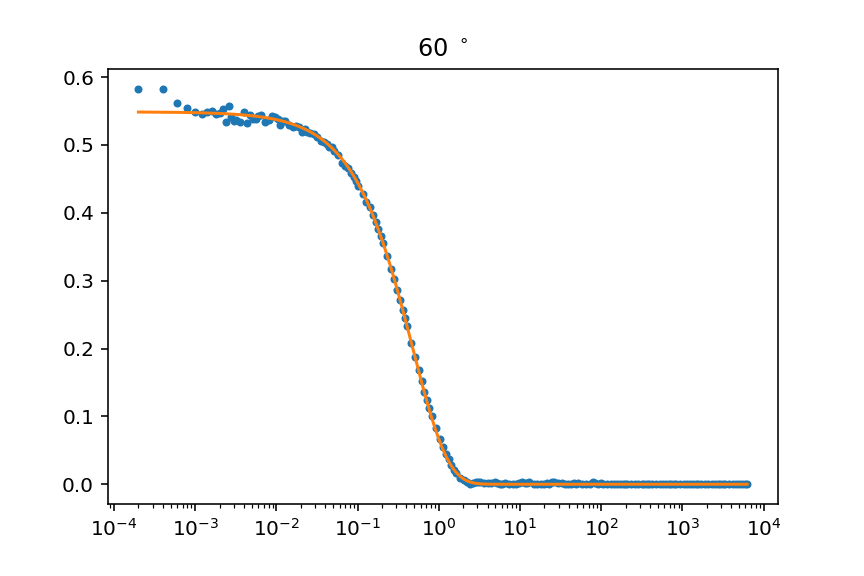
\includegraphics[width=\linewidth]{Plots/A/60.png}
\end{subfigure}
\begin{subfigure}[c]{0.48\linewidth}
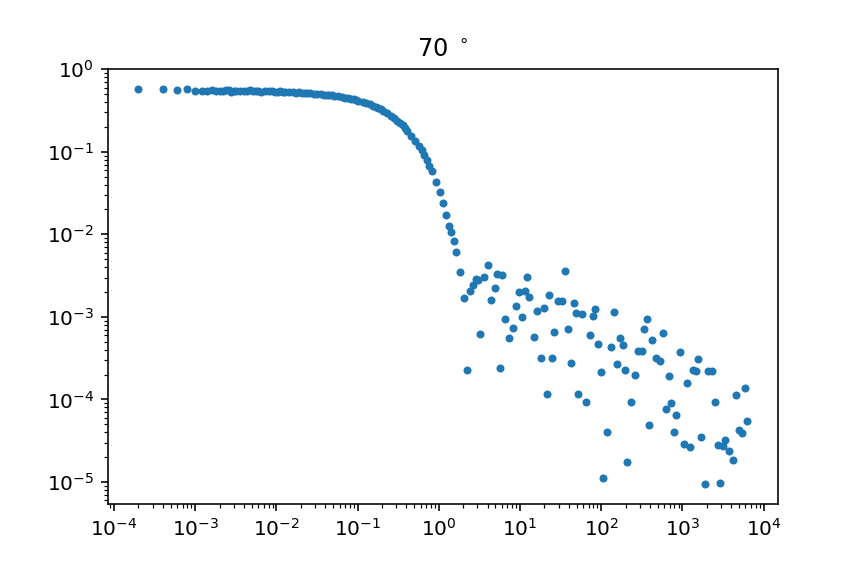
\includegraphics[width=\linewidth]{Plots/A/70.png}
\end{subfigure}

\caption{Autocorrelation Sample A: Angle between 20 and 70 degrees.}
\end{figure}
\newpage

\begin{figure}[!h]
\centering

\medskip
\begin{subfigure}{0.48\textwidth}
\includegraphics[width=\linewidth]{Plots/A/80.png}
\end{subfigure}
\begin{subfigure}[c]{0.48\linewidth}
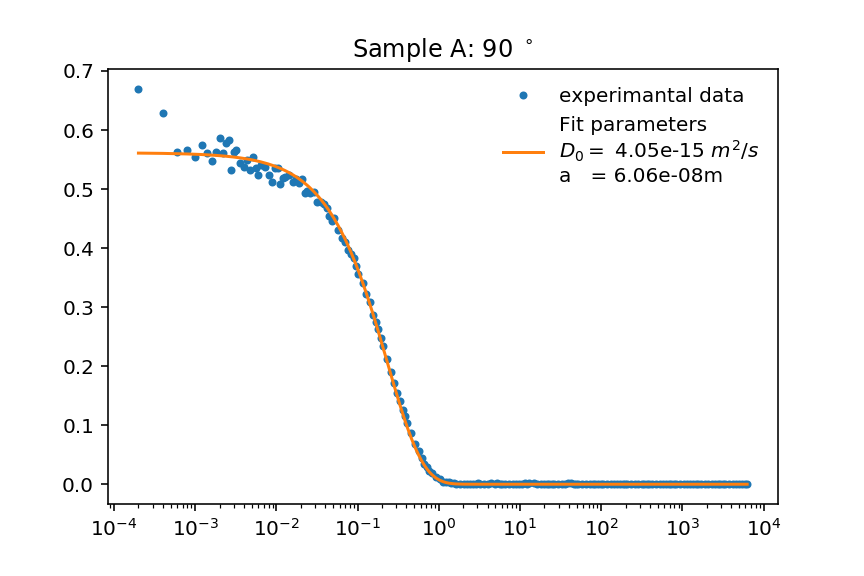
\includegraphics[width=\linewidth]{Plots/A/90.png}
\end{subfigure}

\medskip
\begin{subfigure}{0.48\textwidth}
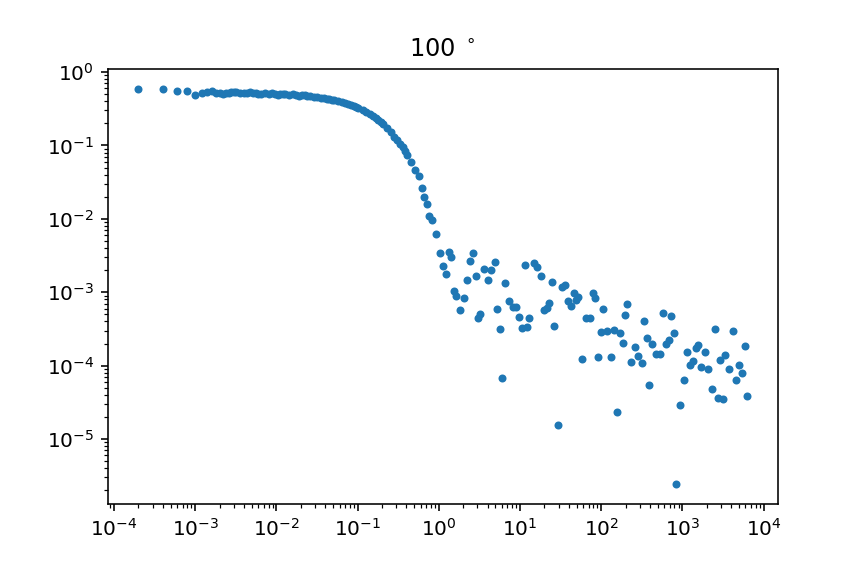
\includegraphics[width=\linewidth]{Plots/A/100.png}
\end{subfigure}
\begin{subfigure}[c]{0.48\linewidth}
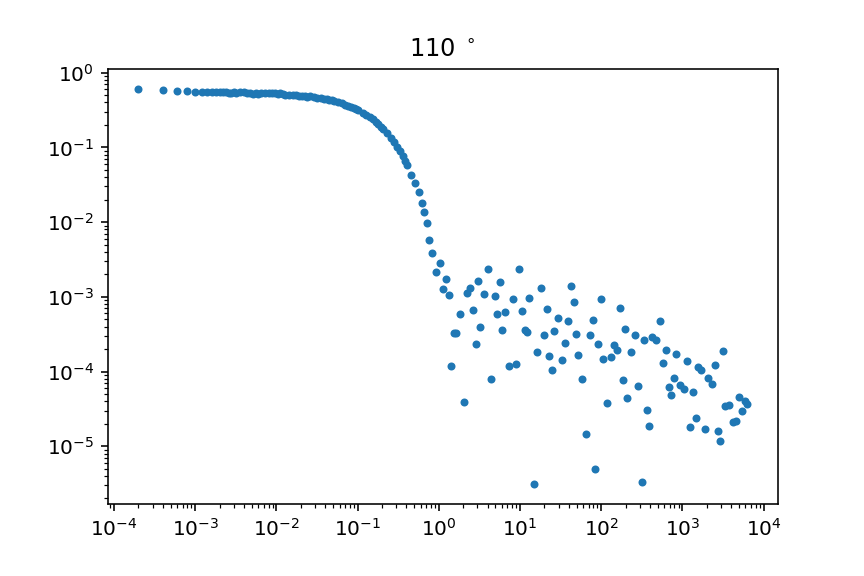
\includegraphics[width=\linewidth]{Plots/A/110.png}
\end{subfigure}

\medskip
\begin{subfigure}{0.48\textwidth}
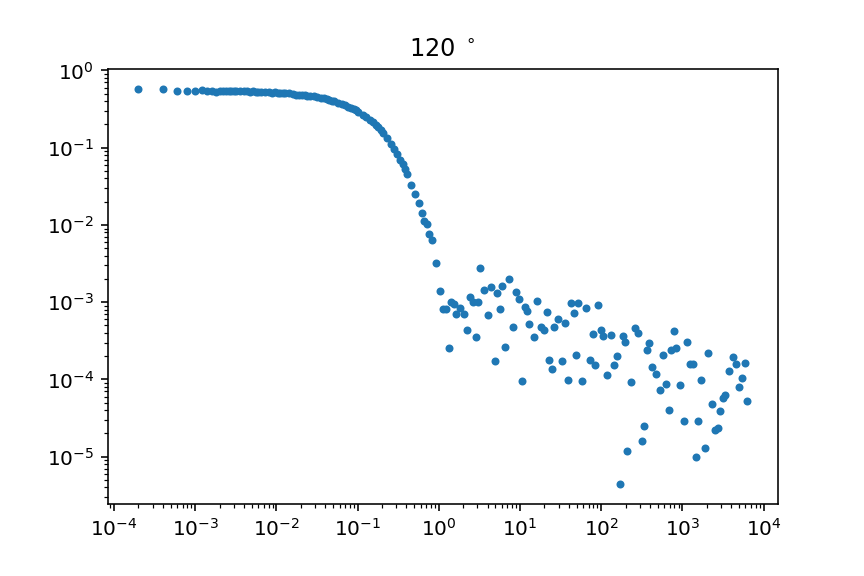
\includegraphics[width=\linewidth]{Plots/A/120.png}
\end{subfigure}
\begin{subfigure}[c]{0.48\linewidth}
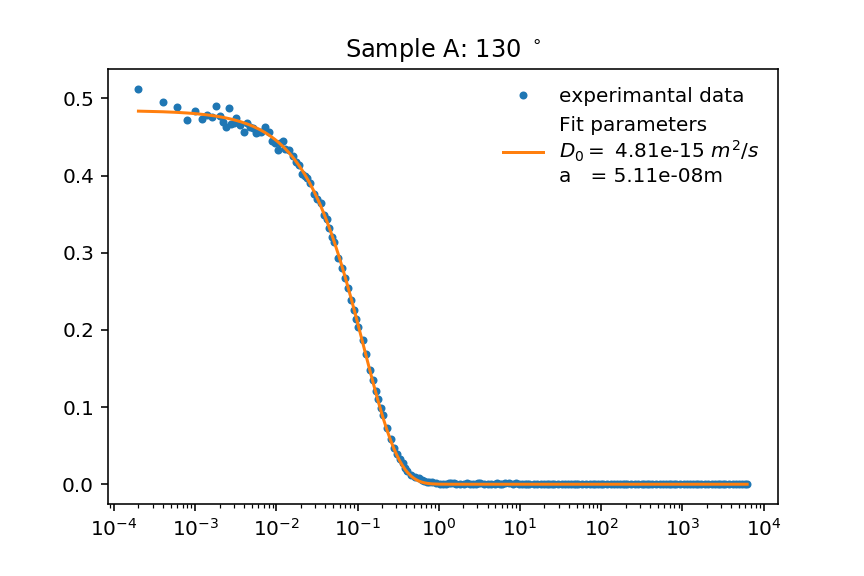
\includegraphics[width=\linewidth]{Plots/A/130.png}
\end{subfigure}

\medskip
\begin{subfigure}{0.48\textwidth}
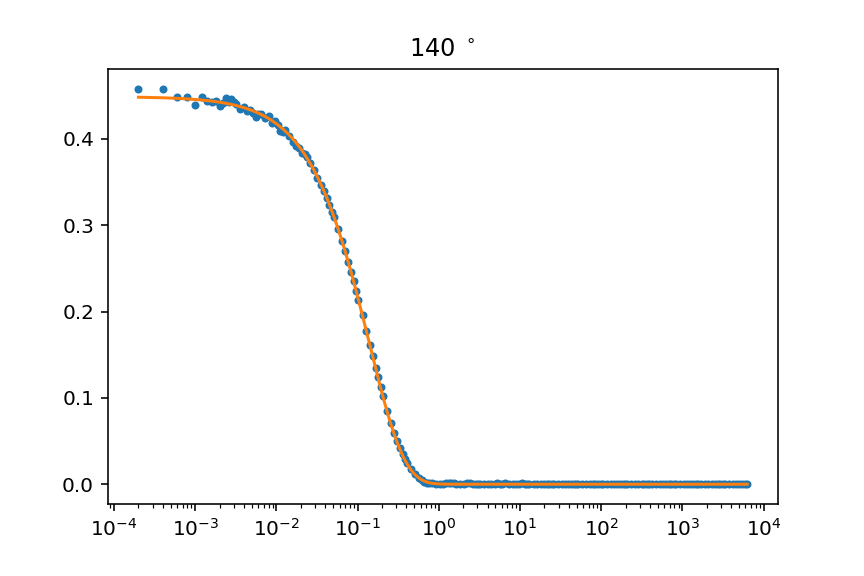
\includegraphics[width=\linewidth]{Plots/A/140.png}
\end{subfigure}
\begin{subfigure}[c]{0.48\linewidth}
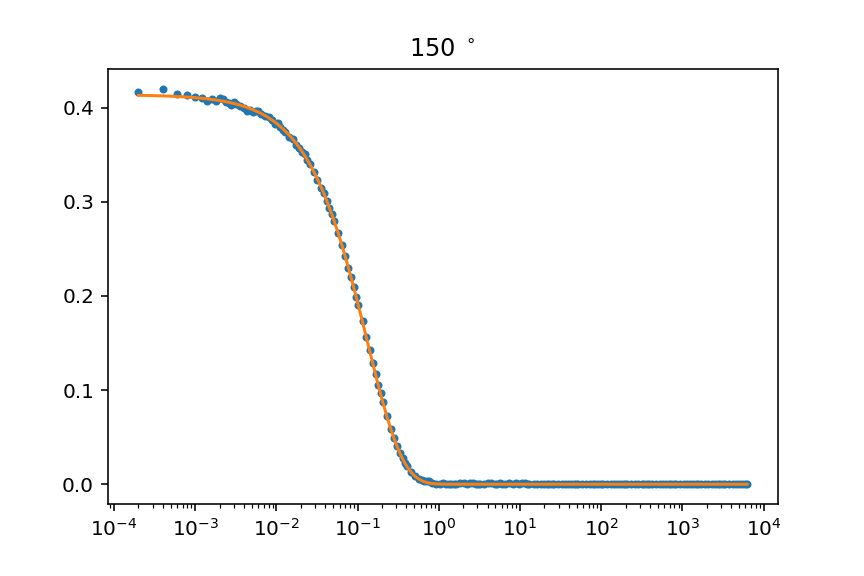
\includegraphics[width=\linewidth]{Plots/A/150.png}
\end{subfigure}

\caption{Autocorrelation Sample A: Angle between 80 and 150 degrees.}
\end{figure}
\newpage

\subsection{Autocorrelation B}
\label{autocorr B}
\begin{figure}[!h]
\centering

\begin{subfigure}{0.48\textwidth}
\includegraphics[width=\linewidth]{Plots/B/20.png}
\end{subfigure}
\begin{subfigure}[c]{0.48\linewidth}
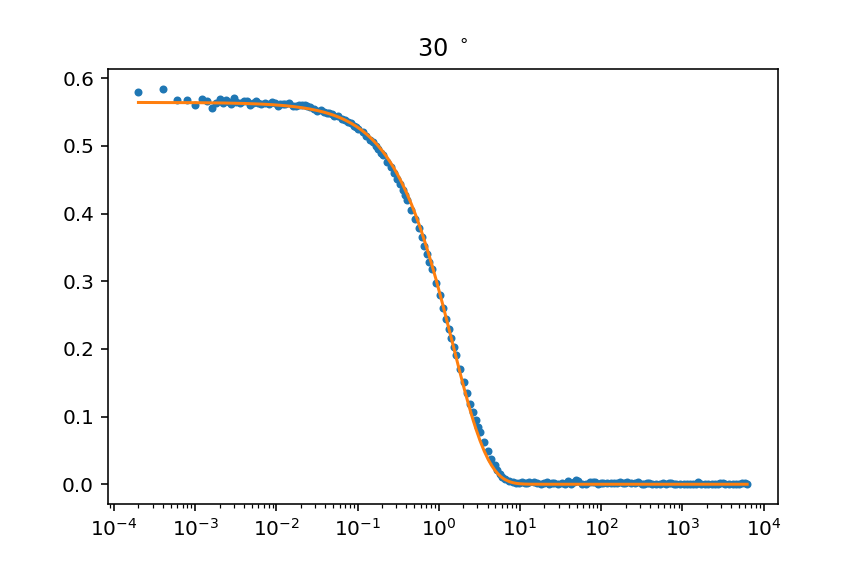
\includegraphics[width=\linewidth]{Plots/B/30.png}
\end{subfigure}

\medskip
\begin{subfigure}{0.48\textwidth}
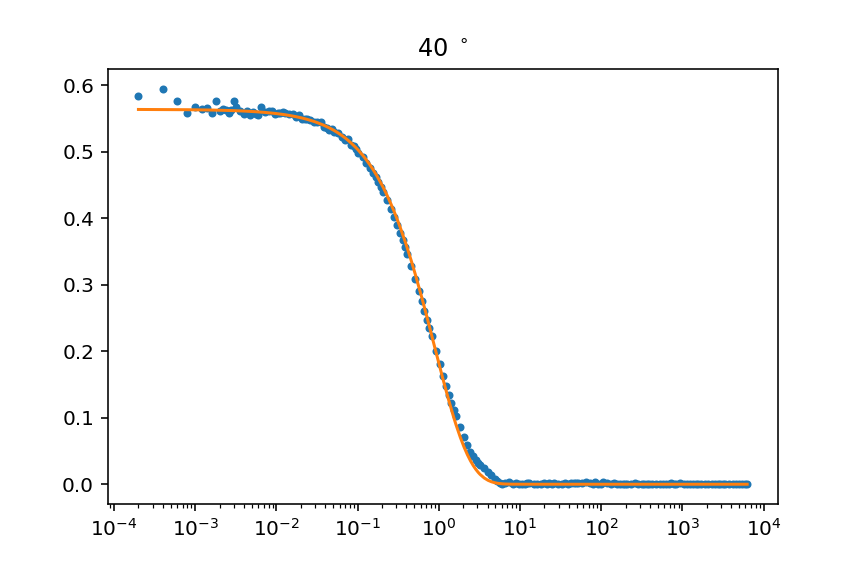
\includegraphics[width=\linewidth]{Plots/B/40.png}
\end{subfigure}
\begin{subfigure}[c]{0.48\linewidth}
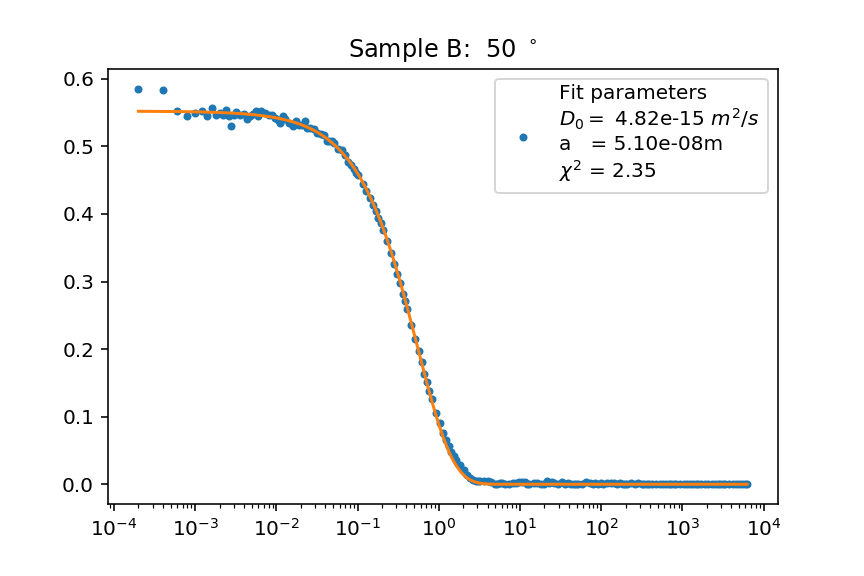
\includegraphics[width=\linewidth]{Plots/B/50.png}
\end{subfigure}

\medskip
\begin{subfigure}{0.48\textwidth}
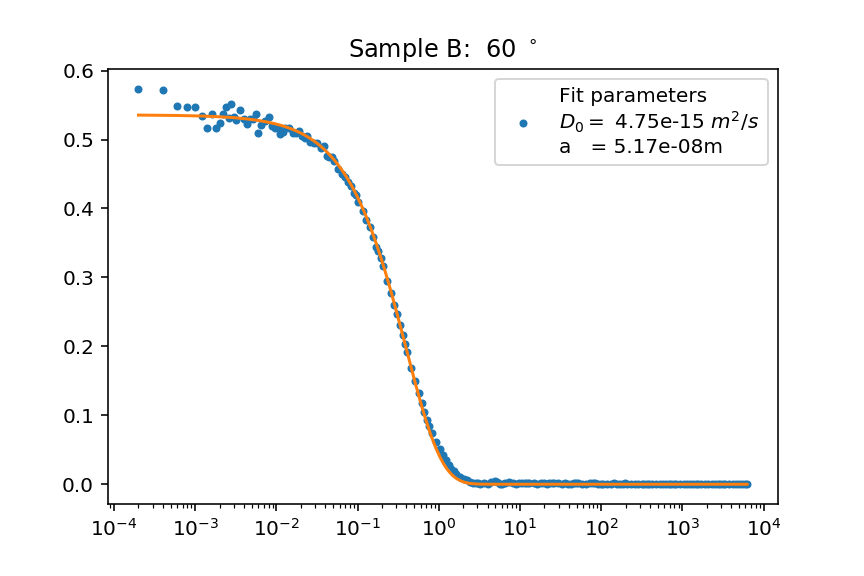
\includegraphics[width=\linewidth]{Plots/B/60.png}
\end{subfigure}
\begin{subfigure}[c]{0.48\linewidth}
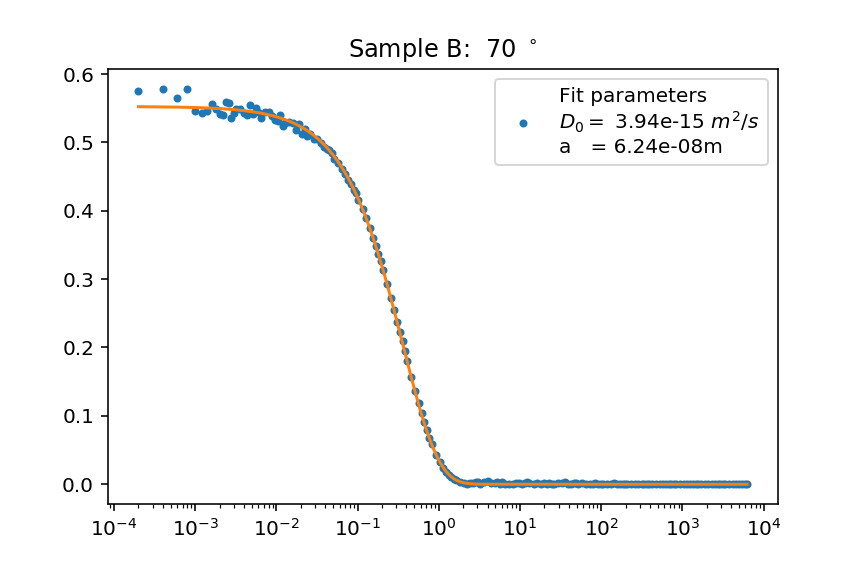
\includegraphics[width=\linewidth]{Plots/B/70.png}
\end{subfigure}

\caption{Autocorrelation Sample B: Angle between 20 and 70 degrees.}
\end{figure}
\newpage

\begin{figure}[!h]
\centering

\medskip
\begin{subfigure}{0.48\textwidth}
\includegraphics[width=\linewidth]{Plots/B/80.png}
\end{subfigure}
\begin{subfigure}[c]{0.48\linewidth}
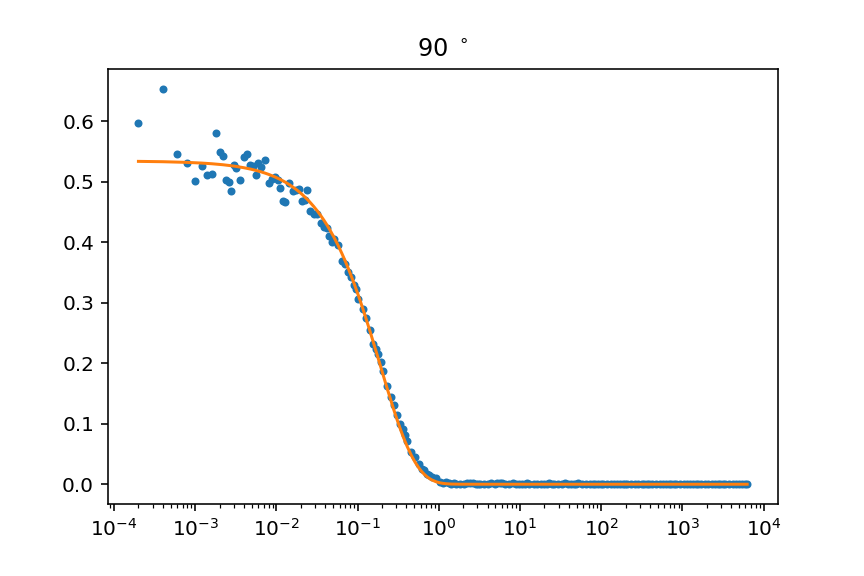
\includegraphics[width=\linewidth]{Plots/B/90.png}
\end{subfigure}

\medskip
\begin{subfigure}{0.48\textwidth}
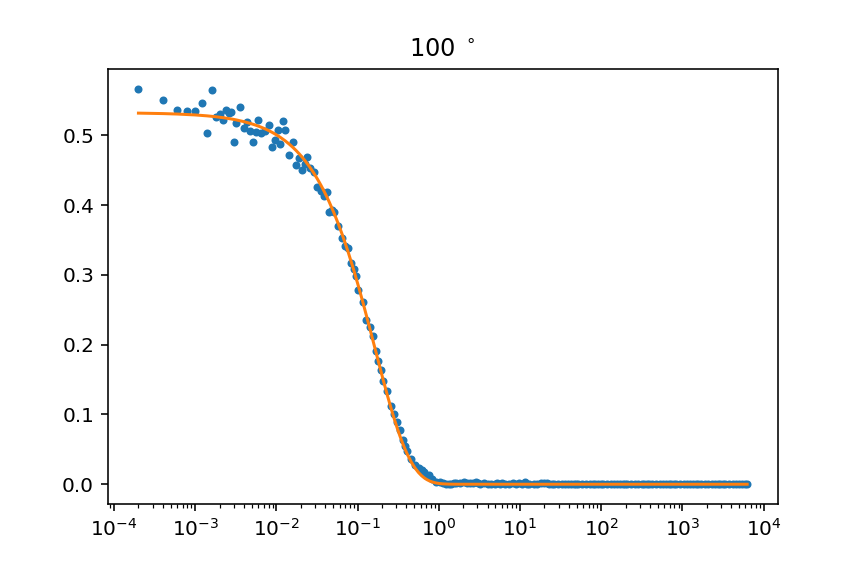
\includegraphics[width=\linewidth]{Plots/B/100.png}
\end{subfigure}
\begin{subfigure}[c]{0.48\linewidth}
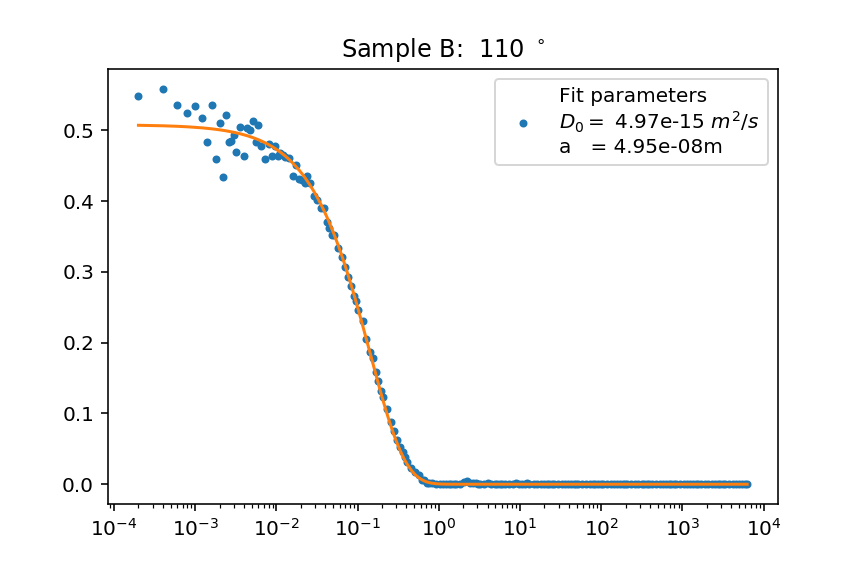
\includegraphics[width=\linewidth]{Plots/B/110.png}
\end{subfigure}

\medskip
\begin{subfigure}{0.48\textwidth}
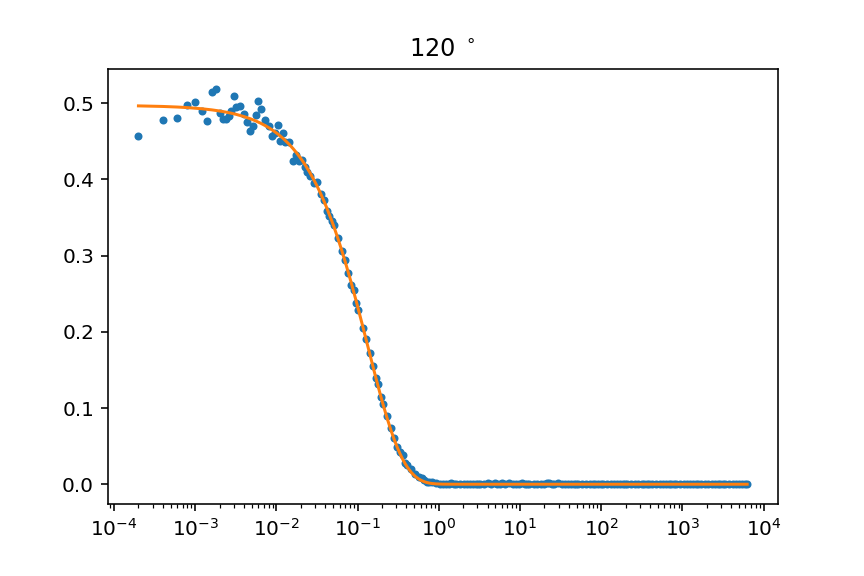
\includegraphics[width=\linewidth]{Plots/B/120.png}
\end{subfigure}
\begin{subfigure}[c]{0.48\linewidth}
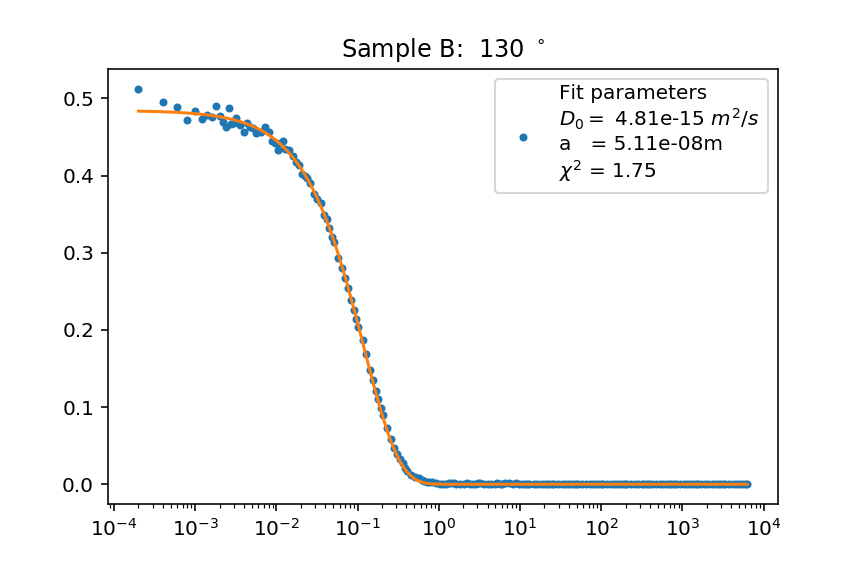
\includegraphics[width=\linewidth]{Plots/B/130.png}
\end{subfigure}

\medskip
\begin{subfigure}{0.48\textwidth}
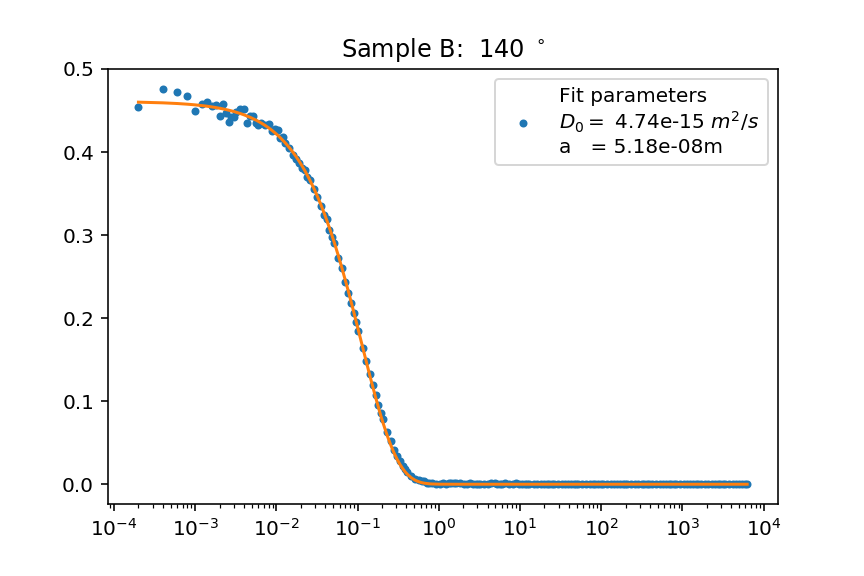
\includegraphics[width=\linewidth]{Plots/B/140.png}
\end{subfigure}
\begin{subfigure}[c]{0.48\linewidth}
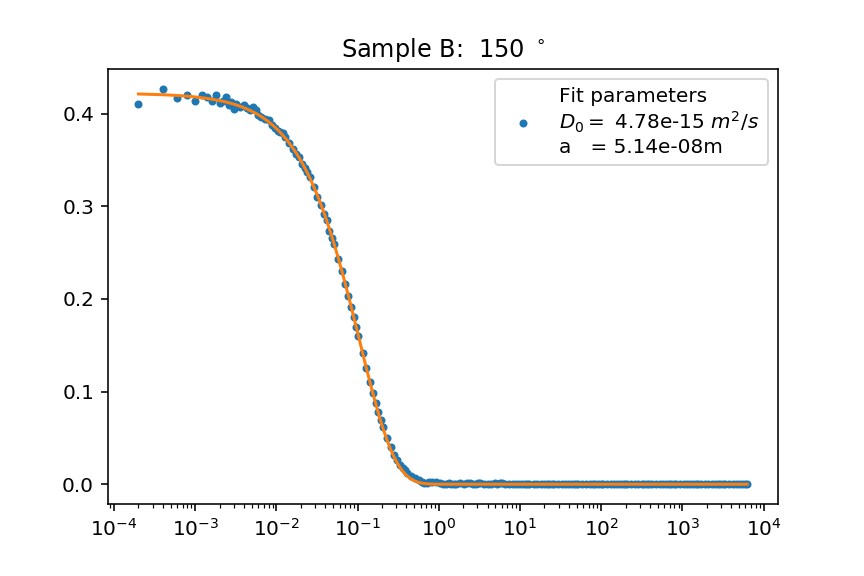
\includegraphics[width=\linewidth]{Plots/B/150.png}
\end{subfigure}

\caption{Autocorrelation Sample B: Angle between 80 and 150 degrees.}
\end{figure}


\newpage
\begin{thebibliography}{}

\bibitem{test} lulululululul

\end{thebibliography}
\end{document}

